\chapter{The Histogram of Gradient Orientations of Signal Plots}
\label{chapter:three}

This Chapter introduces the EEG feature extraction procedure based on the Histogram of Gradient Orientations.  This method is grounded on an extension and modification of the SIFT~\cite{Lowe2004} Descriptor which is used in Computer Vision to extract and map local regions of an image.  At the same time, this Chapter brings to completion the previous one, describing how to mine the information from the Plot and build a feature out of it.

\section{Introduction}

%sinuplot, spectrogram, scalogram

The work of Edelman, Intrator and Poggio~\cite{Edelman1997} on how the visual cortex sense features was the inspiration to the development of an algorithm to identify and decode salient local information from image regions.  The Scale Invariant Feature Transform (SIFT) method is composed of two parts, the SIFT Detector and the SIFT Descriptor.  The first is the procedure to identify relevant areas of an image.  The second is the procedure to describe and characterize a region of an image using the Histogram of Gradient Orientations~\footnote{It should not to be confused with HOG~\cite{Dalal2005}, the Histogram Of Gradients which is another method from Computer Vision based on similar ideas.  Actually, the descriptor part of the SIFT Method has no specific name, but as it is based on building a histogram of gradient orientations, that is the reason why it is described here in that way. }.  The SIFT algorithm is biomimetically inspired in how the visual cortex detects shapes by analyzing orientations~\cite{Edelman1997}.  The patch description is also based on the Theory of Receptive Fields and other related ideas~\cite{Lindeberg2013}.

\section{Feature Extraction: Histogram of Gradient Orientations}
\label{SIFT}

The basic procedure is composed of,

\begin{enumerate}
\item Keypoints $\gls{kp}$ are located on an image of a signal plot.
\item A region of an image, a patch, is located using keypoints as centers.  Each patch has a horizontal $\gls{St}$ and vertical scale $\gls{Sv}$, which determines the size in pixels $\gls{Sx}$ and $\gls{Sy}$,  along the horizontal and vertical axis respectively. 
\item Form each patch, a descriptor $\gls{d}$ is derived which is used as a representation of the graphical information contained within the patch.
\end{enumerate}

On the image generated by the procedure detailed in previous Chapter, a keypoint $\gls{kp}$ is placed on a pixel $(x_{kp}, y_{kp})$ over the image plot and a window around the keypoint is considered. A local image patch of size $\gls{Sx} \times \gls{Sy}$ pixels is constructed by dividing the window in $16$ blocks. It is arranged in a $4 \times 4$ grid and the pixel $\gls{kp}$ is the patch center.  Figure~\ref{fig:sampledescriptor}(a) shows a plot of a signal, a keypoint in red at the center and the surrounding patch.

%TODO Check appendix for details on the modification of the SIFT method.

A local representation of the signal shape within the patch can be described by obtaining the gradient orientations on each of the $16$ blocks and creating a histogram of gradients.  In order to calculate the histogram, the interval $[0-360]$ of possible angles is divided in $8$ bins, each one at $45$ degrees.

Hence, for each spacial bin $ i,j = \{0,1,2,3\} $, corresponding to the indexes of each block $B_{i,j}$,  the orientations are accumulated in a  $3$-dimensional histogram $h$ through the following equation: 
 

\begin{equation}
 h(\theta,i,j) = \sum_{\mathbf{p}} \omega_\mathrm{ang}(\angle J(\mathbf{p}) - \theta)\, \omega_{ij}\left(\mathbf{p} - \mathbf{kp} \right)\, |J(\mathbf{p})|
\label{eq:histogram}
\end{equation}

\noindent  where $\mathbf{p}$ is a pixel from within the patch,  $\theta$ is the angle bin with $ \theta \in \{0, 45, 90, 135, 180, 225, 270, 315\} $,  $ |J(\mathbf{p})| $ is the norm of the gradient vector in the pixel $\mathbf{p}$ and it is computed using finite differences and $\angle J(\mathbf{p}) $ is the angle of the gradient vector.  The scalar $ \omega_\mathrm{ang}(\cdot) $  and vector $ \omega_{ij}(\cdot) $ functions are linear interpolations used by~\cite{Lowe2004} and \cite{Vedaldi2010} to provide a weighting contribution to eight adjacent bins.  They are calculated as  

\begin{equation}
 \omega_{ij}(\mathbf{v}) = \omega( \frac{v_x - x_i}{3 \; \sqrt{2} \; \gls{St}} ) \omega( \frac{v_y - y_i}{3 \; \sqrt{2} \; \gls{Sv}} ) 
\label{eq:ij}
\end{equation}

\begin{equation}
 \omega_\mathrm{ang}(\alpha) = \sum_{r=-1}^{1} \omega( \frac{8\alpha}{2\pi} + 8r)
\label{eq:wang}
\end{equation}

\noindent where $x_i$ and $y_i$ are the spatial bin centers located in $ x_i,y_i = \{-\frac{3}{2},-\frac{1}{2},\frac{1}{2},\frac{3}{2}\} $. The function parameter $\mathbf{v} = ( v_x, v_y ) $ is a vector variable and $\alpha$ a scalar variable.  On the other hand, $r$ is an integer that can vary freely between $\left[ -1,1  \right] $ and allows the argument $\alpha$ to be unconstrained in terms of its values in radians. The interpolating function $\omega(\cdot)$ is defined as:

\begin{equation}
\omega(z) = \max(0,|z|-1).
\label{eq:weighting}
\end{equation}

These binning functions conform a trilinear interpolation that has a combined effect of sharing the contribution of each oriented gradient between their eight adjacent bins in a tridimensional cube in the histogram space, and zero everywhere else.

Lastly, the fixed value of $ 3 $ on Equation~\ref{eq:ij} is a magnification factor, a fixed parameter.  The multiplication by $\sqrt{2}$ on the same equation is related to the unit length of the patch $\gls{Deltas}$ which is described in the section~\ref{patchgeometry}.   As the patch has  $16$ blocks and  $8$ bin angles are considered, a feature $\gls{d}$ called \textit{descriptor} of $128$ dimension is obtained. This technique is a modification of Lowe's SIFT Descriptor method.
%It can be observed that the histogram is computed by multiplying by $ |J(\mathbf{p})| $, so the method considers both, the magnitude and the orientation of the gradient vector. 

Figure~\ref{fig:sampledescriptor} shows an example of a patch and a scheme of the histogram computation. In (A) a plot of the signal and the patch centered around the keypoint is shown. In (B) the possible orientations on each patch are illustrated.  Only the upper-left four blocks are visible.  The first eight orientations of the first block, are labeled from $1$ to $8$ clockwise. The orientations of the second block $ B_{1,2} $ are labeled from $9$ to $16$.  This labeling continues left-to-right, up-down until the eight orientations for all the sixteen blocks are assigned. They form the corresponding $\mathbf{kp}$-descriptor of $128$ coordinates. Finally, in (C) an enlarged image plot is shown where the oriented gradient vector for each pixel can be seen.

\begin{figure}[h!]
\centering
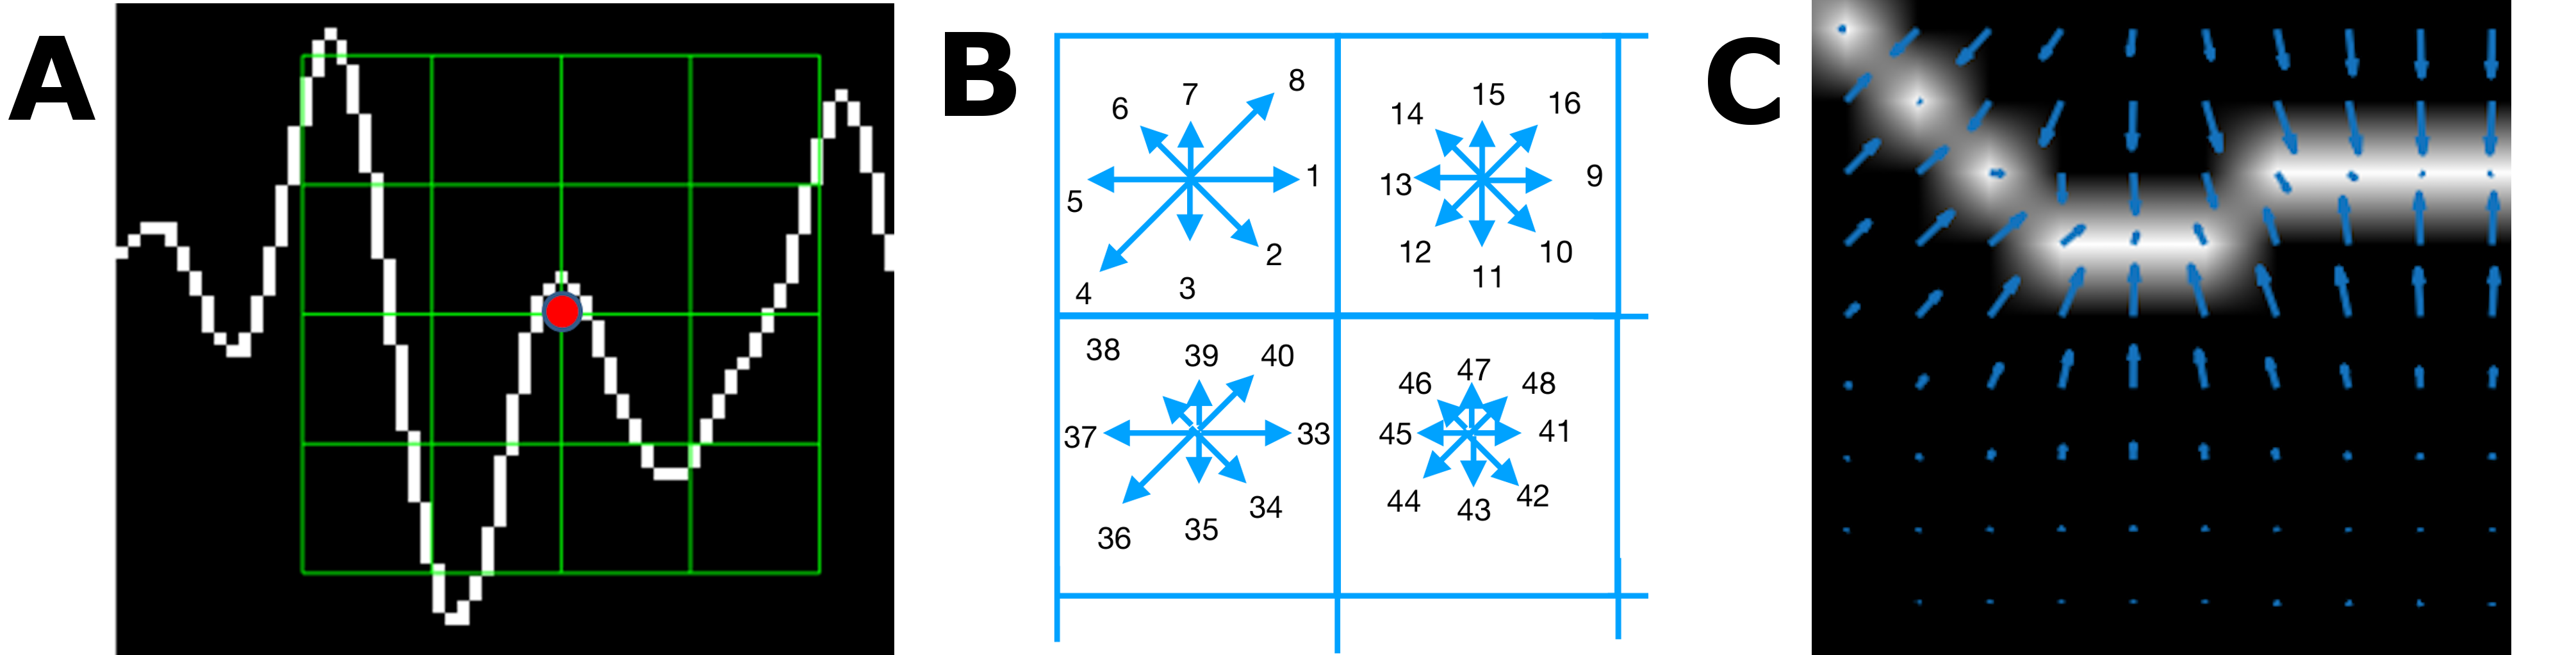
\includegraphics[width=16cm]{images/gradients.png}\label{samplegradients}
\caption[Histogram of Gradient Orientations for ERP]{ (A) Example of a plot of the signal, a keypoint and the corresponding patch. (B) A scheme of the orientation's histogram computation.  Only the upper-left four blocks are visible.  The first eight orientations of the first block, are labeled from $1$ to $8$ clockwise. The orientation of the second block $ B_{1,2} $ is labeled from $9$ to $16$.  This labeling continues left-to-right, up-down until the eight orientations for all the sixteen blocks are assigned. They form the corresponding descriptor of $128$ coordinates.  The length of each arrow represent the value of the histogram on each direction for each block. (C) Vector field of oriented gradients.  Each pixel is assigned an orientation and magnitude calculated  using finite differences. }
\label{fig:sampledescriptor}
\end{figure}

%\begin{figure}[h!]
%\centering
%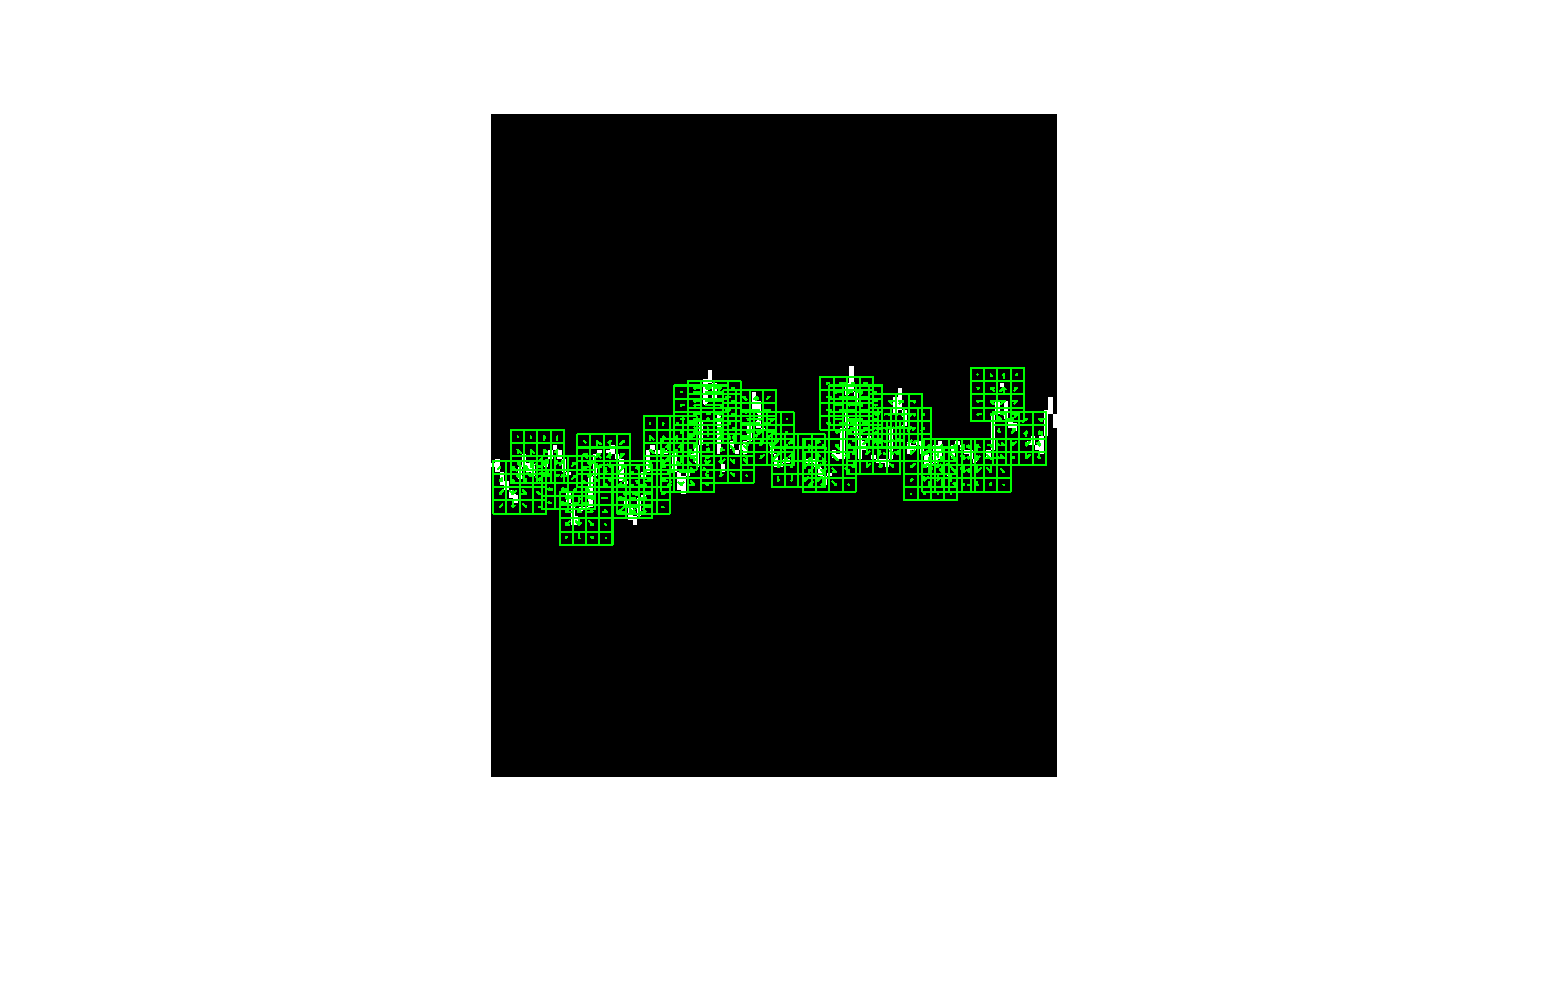
\includegraphics[scale=0.6]{images/KeypointLocations.eps}
%\caption[SIFT Patches]{fdsfdfsfs }
%\label{fig:siftpatch}
%\end{figure}


\section{Keypoint Location}
\label{keypointlocation}

%TODO Vertidal: Along the signal or zero level.
% Horizontal: based on a cognitive event, one or many.
%


The keypoint $\gls{kp}$ location must be accurately specified in order to establish the region from the signal where the waveform is located.

For the horizontal position, the localization of the keypoint is based on a priori information, based on the characteristics of the event under study.  For instance, ERPs have a specific timing that can be explored to elucidate in which position the expected signal pattern will be generated.

Additionally, there can be more than just one keypoint and patch located over the signal plot.  This is particular important for oscillatory processes where many waveforms are contained within the same signal segment.  This needs to be addresses by defining a keypoint density parameter $\gls{kpd}$.

\begin{figure}[h!]
\centering
\subfigure[Fixed size patches are located all along the EEG signal trace at a given keypoint density $\gls{kpd}$.]
{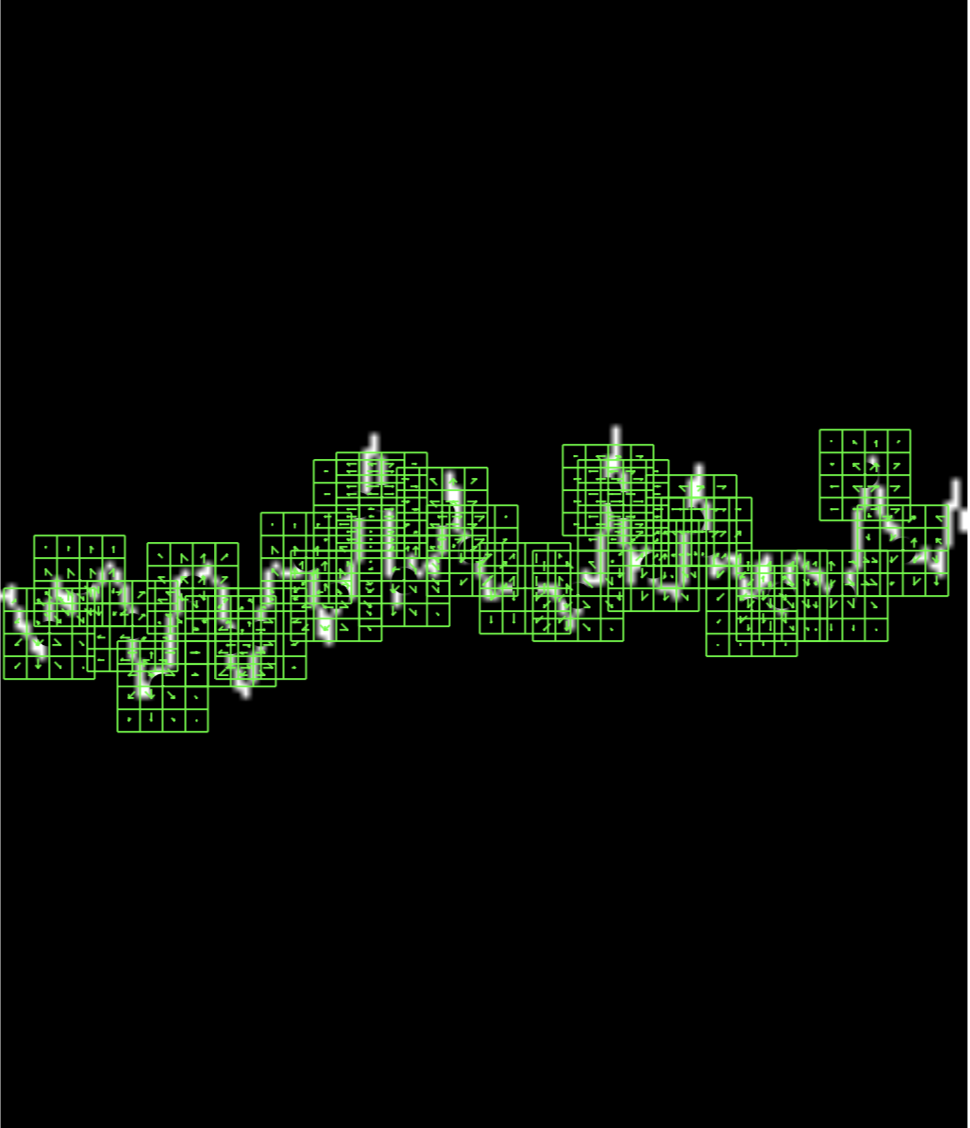
\includegraphics[width=6cm, height=6cm]{images/SignalWithFullDescriptors3.png}}
\subfigure[A patch is used to map an artificial signal using an autoscale plotting scheme, and mapping the entire waveform within the patch. The keypoint is located on the zero-level $z(c)$ value.]
{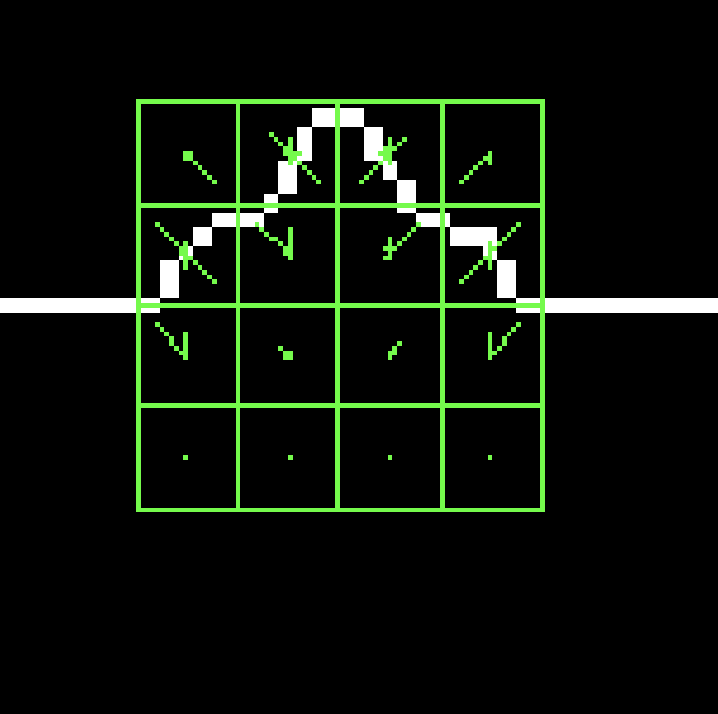
\includegraphics[width=6cm, height=6cm]{images/EasyDescriptorSample3.png}}
\subfigure[Only one fixed size patches are used on a very specific position of the signal trace.]
{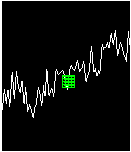
\includegraphics[width=6cm, height=6cm]{images/SignalWithDescriptorSample1.png}}
\subfigure[An entire signal is mapped with fixed size patches with a very high keypoint density $\gls{kpd}$.]
{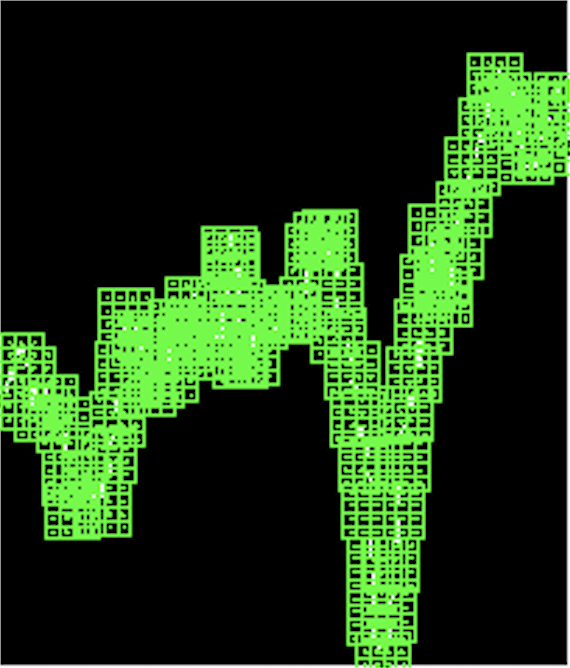
\includegraphics[width=6cm, height=6cm]{images/SignalWithFullDescriptors2.png}}
\caption[Keypoint Locations]{Four different alternatives of keypoint locations and patch geometry.}.
\label{fig:keypointlocations}
\end{figure}

Regarding the Vertical Location, there are two options.  The first one is along the signal, exactly on the sample points calculated by the Equation \ref{eq:images}.  The second is on a fixed position over the zero-level as described by \ref{eq:zerolevel}.  Figure~\ref{fig:keypointlocations}(a) show the former while on (b) the latter can be spotted.

\section{Patch Geometry}
\label{patchgeometry}

%TODO Vertical size: Fixed for autoscaled and variable.
% Horizontal: based on a priori information

The Horizontal Patch Scale $\gls{St}$ determines the size of the patch on the image horizontal axis, and it is related to the span $\gls{lambda}$ of the waveform to analyze according to

\begin{equation}
\gls{St} = \frac{ \gls{lambda} \;  \  \gls{Fs} \ \gls{gammat} }{\gls{Deltas}}
\label{eq:horizontalpatchscale}
\end{equation}

\noindent where $\gls{Fs}$ is the sample frequency, $\gls{gammat}$ is the time scale factor and $\gls{Deltas}$ is the unit length of the patch which determines the pixel conversion factor.  This value depends on the actual implementation of the Histogram of Gradient Orientations of the SIFT method. In this case, its value is $\gls{Deltas} = \sqrt{2} \; 3 \; 5$, where $3$ is the fixed magnification factor.  

On the other hand, on the vertical axis, the vertical patch scale depends on the peak-to-peak amplitude $\gls{DeltamuV}$, and the amplitude scale factor $\gls{gamma}$, as

\begin{equation}
\gls{Sv} = \frac{\gls{DeltamuV} \ \gls{gamma}}{\gls{Deltas}}.
\label{eq:verticalpatchscale}
\end{equation}

The vertical scale can be dynamically adjusted according to the peak-to-peak amplitude of each segment, or it can be set fixed.  This is more appropiate if the underlying signal is bounded which is the case if the standardized procedure described in \ref{standardized} is applied.

\begin{figure}[h!]
\centering
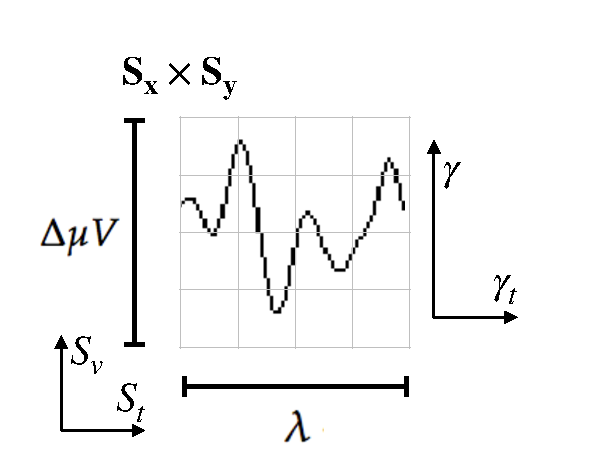
\includegraphics[width=10cm]{images/patchgeometry.pdf}
\caption[Patch Geometry]{The scale of local patch is selected in order to capture the whole transient event.  The size of the patch is $\gls{Sy} \times \gls{Sx}$ pixels. The vertical size consists of $4$ blocks of size $\gls{Sy}$ pixels which should be high enough as to contain the signal $\gls{DeltamuV}$, the peak-to-peak amplitude of the signal component. The horizontal size includes $4$ blocks up to $\gls{Sx}$ and should covert the entire duration in seconds of the signal waveform, $ \gls{lambda} $.   }
\label{fig:patchgeometry}
\end{figure}

Figure~\ref{fig:patchgeometry} shows the different parameters of the patch and how they are related to the underlying signal. Once these parameters are set, the size in pixels of the patch can be obtained in both dimensions.  Hence, the Horizontal Patch Size in pixels is

\begin{equation}
\gls{Sx} = \gls{Deltas} \; \gls{St} + 1.
\label{eq:sx}
\end{equation}

On the other hand, the vertical patch size in pixels can be calculated from

\begin{equation}
\gls{Sy} = \gls{Deltas} \; \gls{Sv} + 1
\label{eq:sy}
\end{equation}

\noindent where $\gls{Deltas}$ being the unit length of the patch. The parameters $\gls{St}$  and $\gls{Sv}$ are the horizontal and vertical patch scale. This region is arranged in a $4 \times 4$ grid and the pixel $\gls{kp}$ is the patch center.   For instance, for a given set of values of $\gls{Sv} = 1$ and $\gls{St} = 1$, the patch is a squared region on the image of size $22$ pixels.

The patch size cannot be bigger than the image itself, whose width is $\gls{Wx}$ and its height is $\gls{Hy}$ .  This is reflected by the following two inequalities that restrict the size of the patch according to 

\begin{equation}
\frac{\gls{Wx}-1}{\gls{Deltas}}  \geq \gls{St} ,
\label{eq:restriction1}
\end{equation}

\noindent on the horizontal axis, and on the vertical axis, 

\begin{equation}
\frac{\gls{Hy}-1}{\gls{Deltas}}  \geq \gls{Sv}.
\label{eq:restriction2}
\end{equation}

\subsection{Oscillatory Processes}

For these patterns, the central idea is to locate keypoints, and their patches, all along the signal trace, filling the entire signal segments with all the possible patches.  In this case, the keypoint density $\gls{kpd} $ determines the step at which a keypoint is located along the trace of the signal, unit sample after unit sample. Care must be taken close to the margins, where there should be a gap to avoid locating incomplete patches.  This can be observed in Figure~\ref{fig:keypointlocations}(a).

\subsection{Transient Events}

For transient events, descriptors are treated as representatives of the single transient waveforms.  This lead to usually just one keypoint that is located in a meaningful position along the horizontal axis.  Additionally, for autoscale plotting, the zero level can be used to localize keypoints.

\section{Classification}
\label{nbnn}

A discriminative~\cite{WolpawJonathanR2012} semi-supervised classification method based on Naive Bayes Nearest Neighbor (NBNN)~\cite{Boiman2008} is applied to classify EEG signals using the features provided by the calculated descriptors.
One problem that frequently arises when using local features is how to go back from the classification of those local characteristics to the image where those descriptors come from.
The NBNN technique overcomes this problem by comparing each image against a whole label class which is characterized by the set of descriptors $q$ that are closest to each one of the descriptors of the query image $\gls{d}_i$. This algorithm is very easy to implement, and is based on the following Equation:

\begin{equation}
\hat{L} = \arg \min_{L} \sum_{\mathbf{d_i}^{(bpc)}} \sum_{q \in N_T(\mathbf{d_i}^{(bpc)})}^{} {\left\lVert q -  \mathbf{d_i}^{(bpc)} \right\rVert}  ^{2} .
\label{eq:classification}
\end{equation}

The estimated class label $\hat{L}$ of a query image is calculated as the class label $L$ that minimize the summation of the distance between each descriptor $\mathbf{d_i}^{(bpc)}$ that belongs to the query image and its corresponding near neighbor $N_T(\mathbf{d}^{(bpc)})$  descriptor for each class. Figure~\ref{fig:nbnnclassification} show a scheme of how this classification method works.

The $\gls{bpc}$ is the Best Performing Channel.  This value is determined in the calibration step of the BCI algorithm when the spatial performance is assessed to determine on which channel the performance is maximized~\cite{Chavarriaga2017}.

\begin{figure}[h!]
\centering
\subfigure[]
{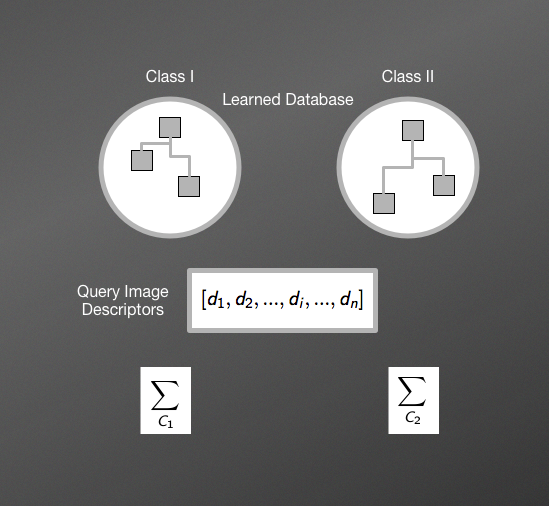
\includegraphics[scale=0.25]{images/NBNNMethod1.png}}
\subfigure[]
{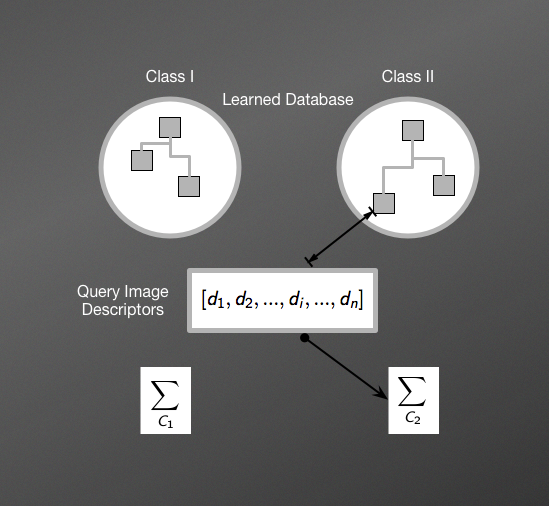
\includegraphics[scale=0.25]{images/NBNNMethod2.png}}
\subfigure[]
{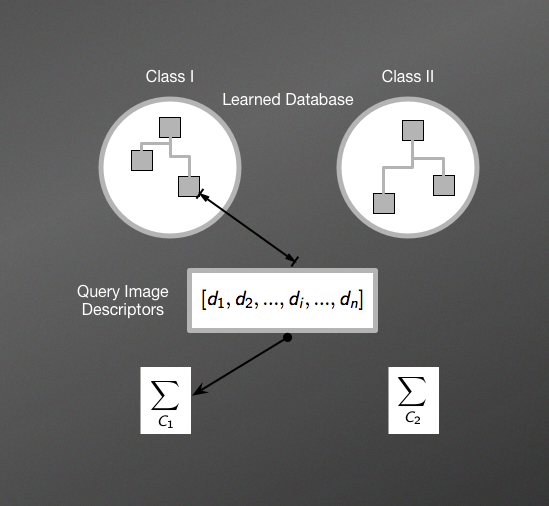
\includegraphics[scale=0.25]{images/NBNNMethod3.png}}
\subfigure[]
{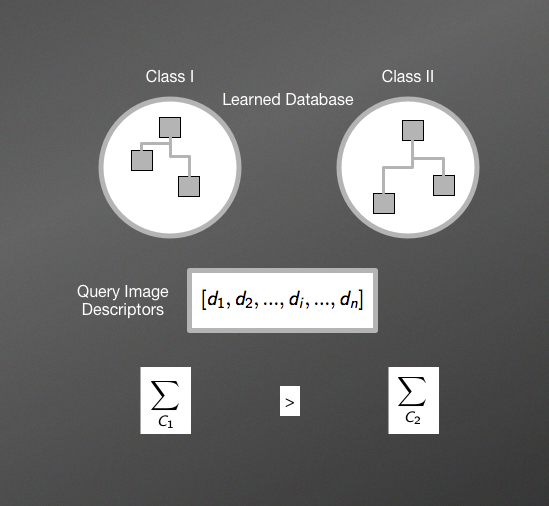
\includegraphics[scale=0.25]{images/NBNNMethod4.png}}
\subfigure[ ]
{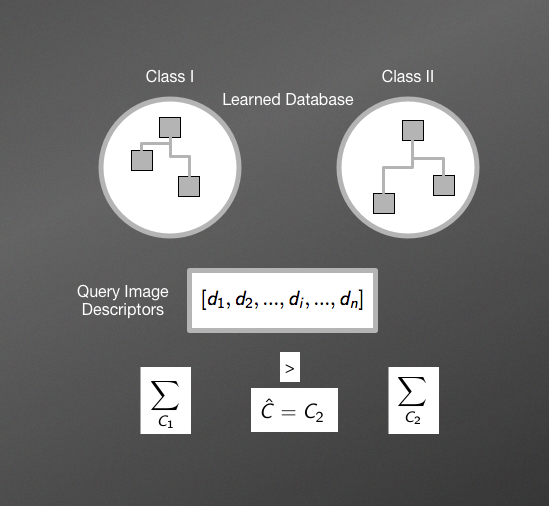
\includegraphics[scale=0.25]{images/NBNNMethod5.png}}
\caption[NBNN Classification]{(a) Two Dictionaries contain templates descriptors for two different classes. A set of query descriptors are extracted from a new image that needs to be categorized.(b) Distances from every descriptor $\gls{d}_i$ are calculated against the closest one from the Dictionary of Class 2.  Distances summations are accumulated.(c) Distance values from every descriptor $\gls{d}_i$ are calculated against the closest one from the Dictionary of Class 1.  Distances summations are accumulated. (d) The two different summation values are compared against each other.(e) The summation that achieved the lesser value is the one that more closely resembles the set of templates, thus is the one predicted by the classification algorithm.}
\label{fig:nbnnclassification}
\end{figure}

%TODO:Agregar tambien las pruebas sobre rootsift y que la distancia mejor es la coseno demostrar justamente haciendo una prueba sobre EEGWave.
%TODO:Agregar que el experimento dio perfecto cuando no se controla la varianza.

\section{BCI Algorithm}

In brief, based on segmented signals from at least two labeled classes, a set of images is first generated.  For each image, keypoints are localized and descriptors are extracted during the training or calibration step of a BCI procedure and they are grouped in KD-tree~\cite{Lowe2004} structures for each one of the classes.  Additionally, the spatial performance is evaluated and the $\gls{bpc}$ value is computed.

Hence, given a new unlabeled signal segment, an image plot is generated as well, their keypoints localized and their descriptors extracted.  They are fed into Equation~\ref{eq:classification} in order to determine the class which minimizes the summation and thus provide the information bit to the BCI controller.  

%\section{Implementation}
%
%\subsection{Software}
%
%The implemented code is published in \url{https://bitbucket.org/itba/hist/} by using Matlab, python and the VLFeat library.
%These algorithm were implemented on MATLAB 2014a (Mathworks Inc., Natick, MA, USA).  To maintain reproducibility, the data and the source code has been made available in the online repository of the Code Ocean platform under the name \textit{EEGWave}.
%
%The algorithm is implemented using  VLFeat~\cite{Vedaldi2010} Computer Vision libraries on MATLAB V2014a (Mathworks Inc., Natick, MA, USA). Furthermore, in order to enhance the impact of our paper and for a sake of reproducibility, the code of the algorithm has been made available at: https://bitbucket.org/itba/hist.

%TODO add the data and also the code ocean repository.  Also add my own repositories.

\section{Implementation Summary}

This section provides a mapping cheat-sheet to convert and obtain the parameters of the algorithm for a given set of signal parameters.

The input signal parameters are $N$,$F_s$, $\lambda$ and the peak-to-peak amplitude $\gls{DeltamuV}$ of the waveform to study. The unit length of the patch is $\Delta_s = \sqrt{2} \; 15$ and as has been earlier mentioned, depends on the particular SIFT implementation.

Output parameters are: 
$\gls{gamma}$
$\gls{gammat}$
$\gls{Hy}$
$\gls{Wx}$
$\gls{St}$
$\gls{Sv}$
$\gls{Sy}$
$\gls{Sx}$
$\gls{kp}$

Mappings:\\

Amplitude scale factor

\begin{align*}
\gamma \equiv \frac{H_y}{\Delta \mu V}  
\end{align*}

Time scale factor

\begin{align*}
\gamma_t \equiv \frac{W_x}{F_s \; w}  
\end{align*}

%\begin{equation}
%s_x = \frac{ \gamma \;  \lambda \  F_s}{12}
%\label{eq:mapping2}
%\end{equation}
%
%\begin{equation}
%s_y= \frac{\gamma \; \Delta \mu V}{12} 
%\label{eq:mapping1}
%\end{equation}

Restriction on the waveform time scale

\begin{align*}
\frac{W_x-1}{\sqrt{2} \; 15}  \geq S_t 
\end{align*}

Restriction on the waveform amplitude scale

\begin{align*}
\frac{H_y-1}{\sqrt{2} \; 15}  \geq S_v 
\end{align*}

Horizontal Patch scale

\begin{align*}
S_t = \frac{ \lambda \;  \  F_s \ \gamma_t }{\Delta_s}
\end{align*}

Vertical Patch scale

\begin{align*}
S_v= \frac{\Delta \mu V \ \gamma}{\Delta_s} 
\end{align*}

Time to sample point conversion

\begin{align*}
n = \left\lfloor F_s \ \Delta_t \right\rfloor \ \gamma_t
\end{align*}

Horizontal Patch size in pixels

\begin{align*}
\mathbf{S}_x = \Delta_s \; S_t + 1
\end{align*}

Vertical Patch Size in pixels

\begin{align*}
\mathbf{S}_y = \Delta_s \; S_v + 1
\end{align*}

Span of a Patch

\begin{align*}
\Delta_t = \frac{S_t \ \Delta_s}{F_s \ \gamma_t} 
\end{align*}
